% Standalone TikZ architecture diagram for AARS
% Can be compiled independently or included in main.tex
\documentclass[border=5mm]{standalone}
\usepackage{tikz}
\usetikzlibrary{shapes.geometric, arrows.meta, positioning, fit, backgrounds}

\begin{document}
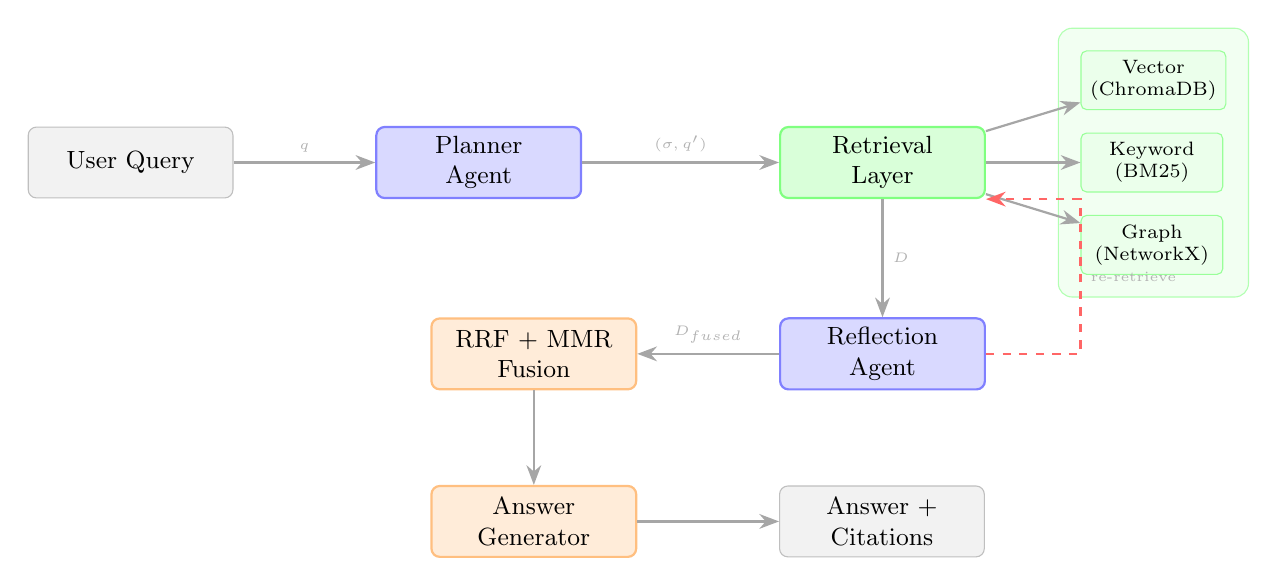
\begin{tikzpicture}[
    node distance=1.2cm and 1.8cm,
    box/.style={rectangle, draw, rounded corners=3pt, minimum width=2.6cm, minimum height=0.9cm, align=center, font=\small},
    agent/.style={box, fill=blue!15, draw=blue!50, thick},
    retriever/.style={box, fill=green!15, draw=green!50, thick},
    process/.style={box, fill=orange!15, draw=orange!50, thick},
    io/.style={box, fill=gray!10, draw=gray!50},
    small/.style={rectangle, draw, rounded corners=2pt, minimum width=1.8cm, minimum height=0.6cm, align=center, font=\scriptsize, fill=green!8, draw=green!40},
    arrow/.style={-{Stealth[length=2.5mm]}, thick, color=gray!70},
    darrow/.style={-{Stealth[length=2.5mm]}, thick, dashed, color=red!60},
    label/.style={font=\tiny, color=gray!60},
]
    % Input/Output
    \node[io] (input) {User Query};

    % Planner
    \node[agent, right=of input] (planner) {Planner\\Agent};

    % Retrieval layer
    \node[retriever, right=2.5cm of planner] (retrieval) {Retrieval\\Layer};

    % Sub-retrievers
    \node[small, above right=0.2cm and 1.2cm of retrieval] (vec) {Vector\\(ChromaDB)};
    \node[small, right=1.2cm of retrieval] (kw) {Keyword\\(BM25)};
    \node[small, below right=0.2cm and 1.2cm of retrieval] (graph) {Graph\\(NetworkX)};

    % Reflection
    \node[agent, below=1.5cm of retrieval] (reflection) {Reflection\\Agent};

    % Fusion
    \node[process, left=of reflection] (fusion) {RRF + MMR\\Fusion};

    % Generator
    \node[process, below=of fusion] (generator) {Answer\\Generator};

    % Output
    \node[io, right=of generator] (output) {Answer +\\Citations};

    % Connections
    \draw[arrow] (input) -- node[above, label] {$q$} (planner);
    \draw[arrow] (planner) -- node[above, label] {$(\sigma, q')$} (retrieval);
    \draw[arrow] (retrieval) -- (vec);
    \draw[arrow] (retrieval) -- (kw);
    \draw[arrow] (retrieval) -- (graph);
    \draw[arrow] (retrieval) -- node[right, label] {$D$} (reflection);
    \draw[darrow] (reflection.east) -- ++(1.2,0) |- node[right, label, pos=0.25] {re-retrieve} (retrieval.south east);
    \draw[arrow] (reflection) -- node[above, label] {$D_{fused}$} (fusion);
    \draw[arrow] (fusion) -- (generator);
    \draw[arrow] (generator) -- (output);

    % Background groups
    \begin{scope}[on background layer]
        \node[fit=(vec)(kw)(graph), draw=green!30, fill=green!5, rounded corners=5pt, inner sep=8pt] {};
    \end{scope}
\end{tikzpicture}
\end{document}
